\documentclass[a4paper,12pt]{article}

%%% Работа с русским языком
\usepackage{cmap}					% поиск в PDF
\usepackage{mathtext} 				% русские буквы в формулах
\usepackage[T2A]{fontenc}			% кодировка
\usepackage[utf8]{inputenc}			% кодировка исходного текста
\usepackage[english,russian]{babel}	% локализация и переносы
\usepackage{comment}


%%% Дополнительная работа с математикой
\usepackage{amsfonts,amssymb,amsthm,mathtools} % AMS
\usepackage{amsmath}
\usepackage{icomma} % "Умная" запятая: $0,2$ --- число, $0, 2$ --- перечисление

%% Номера формул
%\mathtoolsset{showonlyrefs=true} % Показывать номера только у тех формул, на которые есть \eqref{} в тексте.

%% Шрифты
\usepackage{euscript}	 % Шрифт Евклид
\usepackage{mathrsfs} % Красивый матшрифт

\usepackage{extsizes} % Возможность сделать 14-й шрифт
\usepackage{geometry} % Простой способ задавать поля
\geometry{top=25mm}
\geometry{bottom=35mm}
\geometry{left=20mm}
\geometry{right=20mm}

\usepackage{chngcntr}
\usepackage{hyperref}

\usepackage{setspace} % Интерлиньяж
%\onehalfspacing % Интерлиньяж 1.5
%\doublespacing % Интерлиньяж 2
%\singlespacing % Интерлиньяж 1

\usepackage{lastpage} % Узнать, сколько всего страниц в документе.
\usepackage{soulutf8} % Модификаторы начертания

\counterwithin*{equation}{section}
\counterwithin*{equation}{subsection}



%% Свои команды
\DeclareMathOperator{\sgn}{\mathop{sgn}}

%% Перенос знаков в формулах (по Львовскому)
\newcommand*{\hm}[1]{#1\nobreak\discretionary{}
{\hbox{$\mathsurround=0pt #1$}}{}}

%%% Работа с картинками
\usepackage{graphicx}  % Для вставки рисунков
\graphicspath{{images/}{images2/}}  % папки с картинками
\setlength\fboxsep{3pt} % Отступ рамки \fbox{} от рисунка
\setlength\fboxrule{1pt} % Толщина линий рамки \fbox{}
\usepackage{wrapfig} % Обтекание рисунков и таблиц текстом

%%% Работа с таблицами
\usepackage{array,tabularx,tabulary,booktabs} % Дополнительная работа с таблицами
\usepackage{longtable}  % Длинные таблицы
\usepackage{multirow} % Слияние строк в таблице
\usepackage{graphicx}
\usepackage{fancyhdr}
\usepackage{hyperref}
\usepackage{booktabs}

\newcommand{\lt}{\left}
\newcommand{\rt}{\right}
\newcommand{\al}{\alpha}
\newcommand{\p}{\partial}
\newcommand{\D}{\Delta}
\newcommand{\fr}{\frac}
\newcommand{\dfr}{\dfrac}
\newcommand{\mbf}{\mathbf}
\newcommand{\bb}{\mathbb}
\newcommand{\wt}{\widetilde}
\newcommand{\La}{\Lambda}
\newcommand{\la}{\lambda}
\newcommand{\opn}{\operatorname}
\newcommand{\vp}{\varphi}


\pagestyle{fancy}
\fancyhf{}
\pagestyle{plain} % нумерация вкл.

\rhead{\today}
\lhead{Соколов Игорь, группа 573}

%%% Заголовок
\author{Соколов Игорь, группа 573}
\title{ДЗ 7 по Методам Оптимизации. \newline Субградиент. Субдифференциал.}
\date{\today}

\begin{document} % конец преамбулы, начало документа

\maketitle

\section{}

Докажите, что точка $x_0$ - является точкой минимума выпуклой функции $f(x)$ тогда и только тогда, когда $0 \in \partial f(x_0)$

\begin{proof}

$\Longrightarrow$

Имеем:  $x_0$ - точка минимума функции $f(x)$.

Тогда $\forall x \in \bb R^n \leftarrow f(x) - f(x_0) \ge 0$, что можно переписать в виде:

$$f(x) - f(x_0) \ge 0 = \langle 0_n, x - x_0 \rangle \quad  \forall x \in \bb R^n$$

$\Rightarrow 0_n \in \p f(x_0)$

\vspace{\baselineskip}

$\Longleftarrow$

Имеем: $x_0\text{ такова, что } 0_n \in \p f(x_0) $

Тогда по определению субградиента 

$$f(x) - f(x_0) \ge \langle 0_n, x - x_0 \rangle = 0 \quad  \forall x \in \bb R^n$$

Таким образом точка $x_0$ есть точка минимума функции $f(x)$ на $\bb R^n$
\end{proof}

\section{}

Найти $\partial f(x)$, если $f(x) = \text{ReLU}(x) = \max \{0, x\}$

\vspace{\baselineskip}

\textbf{Решение:}

\vspace{\baselineskip}

$\p f = 
\begin{cases}
0,& x < 0\\
1,& x > 0\\
?,& x = 0
\end{cases}
$

Случай $x = 0$ требует более подробного рассмотрения.

Теорема о субдифференциале поточечного максимума:

\textit{
Пусть $f_i(x)$ - выпуклые функции на открытом выпуклом множестве $S  \subseteq \mathbb{R}^n, \; x_0 \in S$, а поточечный максимум определяется как $f(x)  = \underset{i}{\operatorname{max}} f_i(x)$. Тогда:
$$\partial_S f(x_0) = \mathbf{conv}\left\{  \bigcup\limits_{i \in I(x_0)} \partial_S f_i(x_0) \right\}$$
где $I(x) = \{ i \in [1:m]: f_i(x) = f(x)\}$
}

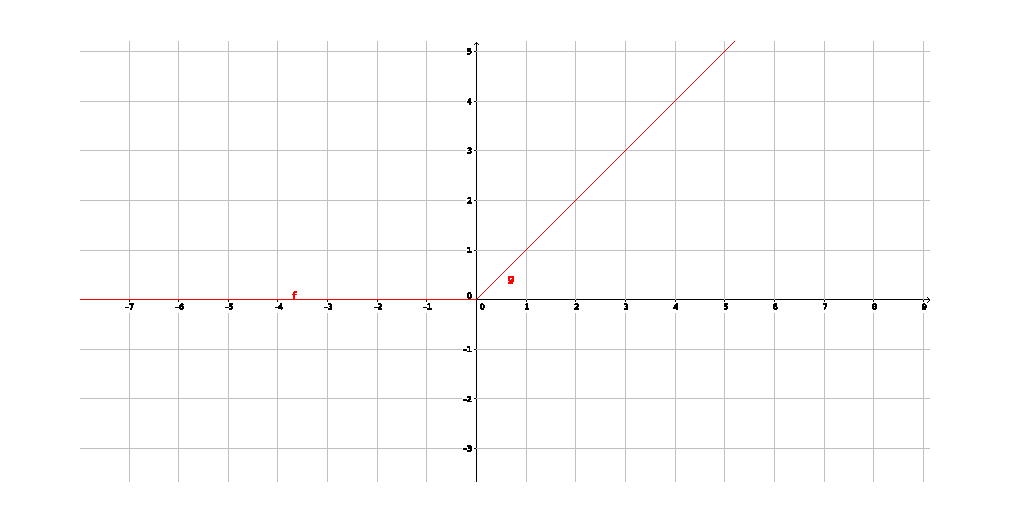
\includegraphics[width=\textwidth]{image1.pdf}

В нашем случае $f_1(x) = 0, \quad f_2(x) = x$ 

$\Rightarrow \p f_1(0) = 0, \quad \p f_2(0) = 1 $


$\Rightarrow \p f(0) = \mbf {conv} \lt\{ \{0\},\{1\} \rt\} = [0, 1]$


\textbf{Ответ:}
$\p f = 
\begin{cases}
0,& x < 0\\
1,& x > 0\\
[0,1],& x = 0
\end{cases}
$

\section{}

Найти $\partial f(x)$, если $f(x) = \|x\|_p$ при $p = 1,2, \infty$

\vspace{\baselineskip}

\textbf{Решение:}

\begin{itemize}
	\item $p = 1$
	
	Применим теорему Моро-Рокафеллара:
	
	\textit {Пусть $f_i(x)$ - выпуклые функции на выпуклых множествах $S_i, \; i = \overline{1,n}$.  
		Тогда, если $\bigcap\limits_{i=1}^n \mathbf{ri } S_i \neq \emptyset$ то функция $f(x) = \sum\limits_{i=1}^n a_i f_i(x), \; a_i > 0$ имеет субдифференциал $\partial_S f(x)$ на множестве $S = \bigcap\limits_{i=1}^n S_i$ и 
		$$\partial_S f(x) = \sum\limits_{i=1}^n a_i \partial_{S_i} f_i(x)$$} 
	
	$ \partial ||{\bf x}||_1 =
	{\bf e_1 } \cdot
	\begin{cases}
	1, & \text{если $x_1 > 0$;} \\
	-1, & \text{если $x_1 < 0$;} \\
	[-1,1], & \text{если $x_1 = 0$.}
	\end{cases}
	+
	{\bf e_2 } \cdot
	\begin{cases}
	1, & \text{если $x_2 > 0$;} \\
	-1, & \text{если $x_2 < 0$;} \\
	[-1,1], & \text{если $x_2 = 0$.}
	\end{cases}
	+\dots+
	$
	
	$ +
	{\bf e_n } \cdot
	\begin{cases}
	1, & \text{если $x_n > 0$;} \\
	-1, & \text{если $x_n < 0$;} \\
	[-1,1], & \text{если $x_n = 0$.}
	\end{cases}
	$
	
	где ${\bf e_i } $ --- единичный орт по оси $\bf 0  x_i$.
	
	\item $p = 2$
	
	$f(x) = \|x\|_2 = \sqrt{\sum\limits_{i = 0}^{n} |x_i|^2 } = \sqrt{x_1^2 + \dots + x_n^2 }$
\begin{itemize}	
	\item $x \neq 0$

	$\forall x \neq 0 \rightarrow f(x)$ является дифференцируемой функцией $$\Rightarrow \p f(x) = \nabla f(x) = \dfr{x}{\|x\|_2}$$ 
	
	\item $x = 0$
	
	По опр:
	$$f(x)\ge f(x_0) + \langle g, x - x_0\rangle$$
	$$\|x\|_2\ge \langle g, x\rangle$$
	$$\lt\langle g, \fr{x}{\|x\|_2}\rt\rangle \le 1 \quad \forall x\in \bb R^n$$
	$$\lt\langle g, e\rt\rangle \le 1$$
	
	$$\lt\langle g, e\rt\rangle \le \|g\|_2\|e\|_2 = \|g\|_2$$
	
	$$\p f = \lt\{g\mid \|g\|_2 \le 1 \quad \forall x\in \bb R^n \rt\}$$
	
\end{itemize}
	\item $p = \infty$
	
	Аналогично можно получить:
	
	$$\lt\langle g, \fr{x}{\|x\|_{\infty}}\rt\rangle \le 1 \quad \forall x\in \bb R^n$$
	
	$$\p f = \lt\{g\mid \|g\|_{\infty} \le 1 \quad \forall x\in \bb R^n \rt\}$$
\end{itemize}


\section{}

Найти $\partial f(x)$, если $f(x) = \|Ax - b\|_1^2$

\vspace{\baselineskip}

\textbf{Решение:}

\begin{itemize}
	
\item $Ax \neq b$

Пусть $A \in \bb R^{n\times m}, x \in \bb R^m$

$\forall x: Ax \neq b \rightarrow$ $f$ является дифференцируемой $\Rightarrow\p f = \nabla f$.

Рассмотрим $f$ как $f(\vp(\psi(g)))$, где 

$f(\vp) = \vp^2$

$\vp(\psi) = \psi^2,$
 
$\psi(g) = \|g\|_1,$ 

$g(x) = Ax-b$

Тогда по правилу нахождения субдифференциала сложной функции:
$$\p f = \fr{\p f}{\p \vp}\fr{\p \vp}{\p \psi}\fr{\p \psi}{\p g}\p g$$

Вспомогательная задача: $\nabla f$, где $f(x) = \|x\|_1 = \sum\limits_{i = 0}^{n}|x_i|$

$$\fr{\p f}{\p x_k} = \sgn(x_k) $$

$$\nabla f = \begin{pmatrix}
\sgn (x_1)\\
\vdots\\
\sgn(x_n)
\end{pmatrix} $$

Также заметим, что $\|Ax-b\|_1 = \sum\limits_{i = 0}^{n}\Big|\sum\limits_{j = 0}^{m}a_{ij}x_j - b_i\Big|$

Тогда $$\p f = 2\|Ax-b\|_1A^{T}
\begin{pmatrix}
\sgn\lt(\sum\limits_{j = 0}^{m}a_{1j}x_j - b_1\rt)\\
\vdots\\
\sgn\lt(\sum\limits_{j = 0}^{m}a_{nj}x_j - b_n\rt)
\end{pmatrix}$$

\item $Ax = b$

По опр:
$$f(x)\ge f(x_0) + \langle g, x - x_0\rangle$$

$x_0 = (A^TA)^{-1}A^Tb$

$$\|Ax - b\|_1^2 \ge \langle g, x - (A^TA)^{-1}A^Tb \rangle$$

\end{itemize}
\section{}

Найти $\partial f(x)$, если $f(x) = e^{\|x\|}$

Рассмотрим $\|x\|_2$.

Аналогично.
\begin{itemize}
	\item $x \neq 0$
	
	Пусть 
	
	$f(g) = e^g$
	
	$g(x) = \|x\|_2$
	
	$$\p f = \fr{\p f}{\p g}\p g$$
	
	$$\p f = e^{\|x\|_2}\fr{x}{\|x\|_2}$$
	
	
	\item $x = 0$
	
	По опр:
	$$f(x)\ge f(x_0) + \langle g, x - x_0\rangle$$
	$$e^{\|x\|_2} - 1\ge \langle g, x\rangle$$
	$$\p f = \lt\{g\Big|  \lt\langle g, \fr{x}{e^{\|x\|_2} - 1}\rt\rangle \le 1 \quad \forall x\in \bb R^n \rt\}$$
	
\end{itemize}

\end{document} % конец документа

